\documentclass[a4paper,landscape]{article}

\usepackage[landscape,top=0cm,left=0cm,bottom=0cm,right=0cm]{geometry}
\usepackage{tikz}
\usepackage{background}
\usepackage{blindtext}
\usetikzlibrary{matrix, shapes.misc, calc}

\pagestyle{empty}
\setlength{\parindent}{0cm}
\backgroundsetup{scale = 1, angle = 0, opacity = 1, color=black, contents = {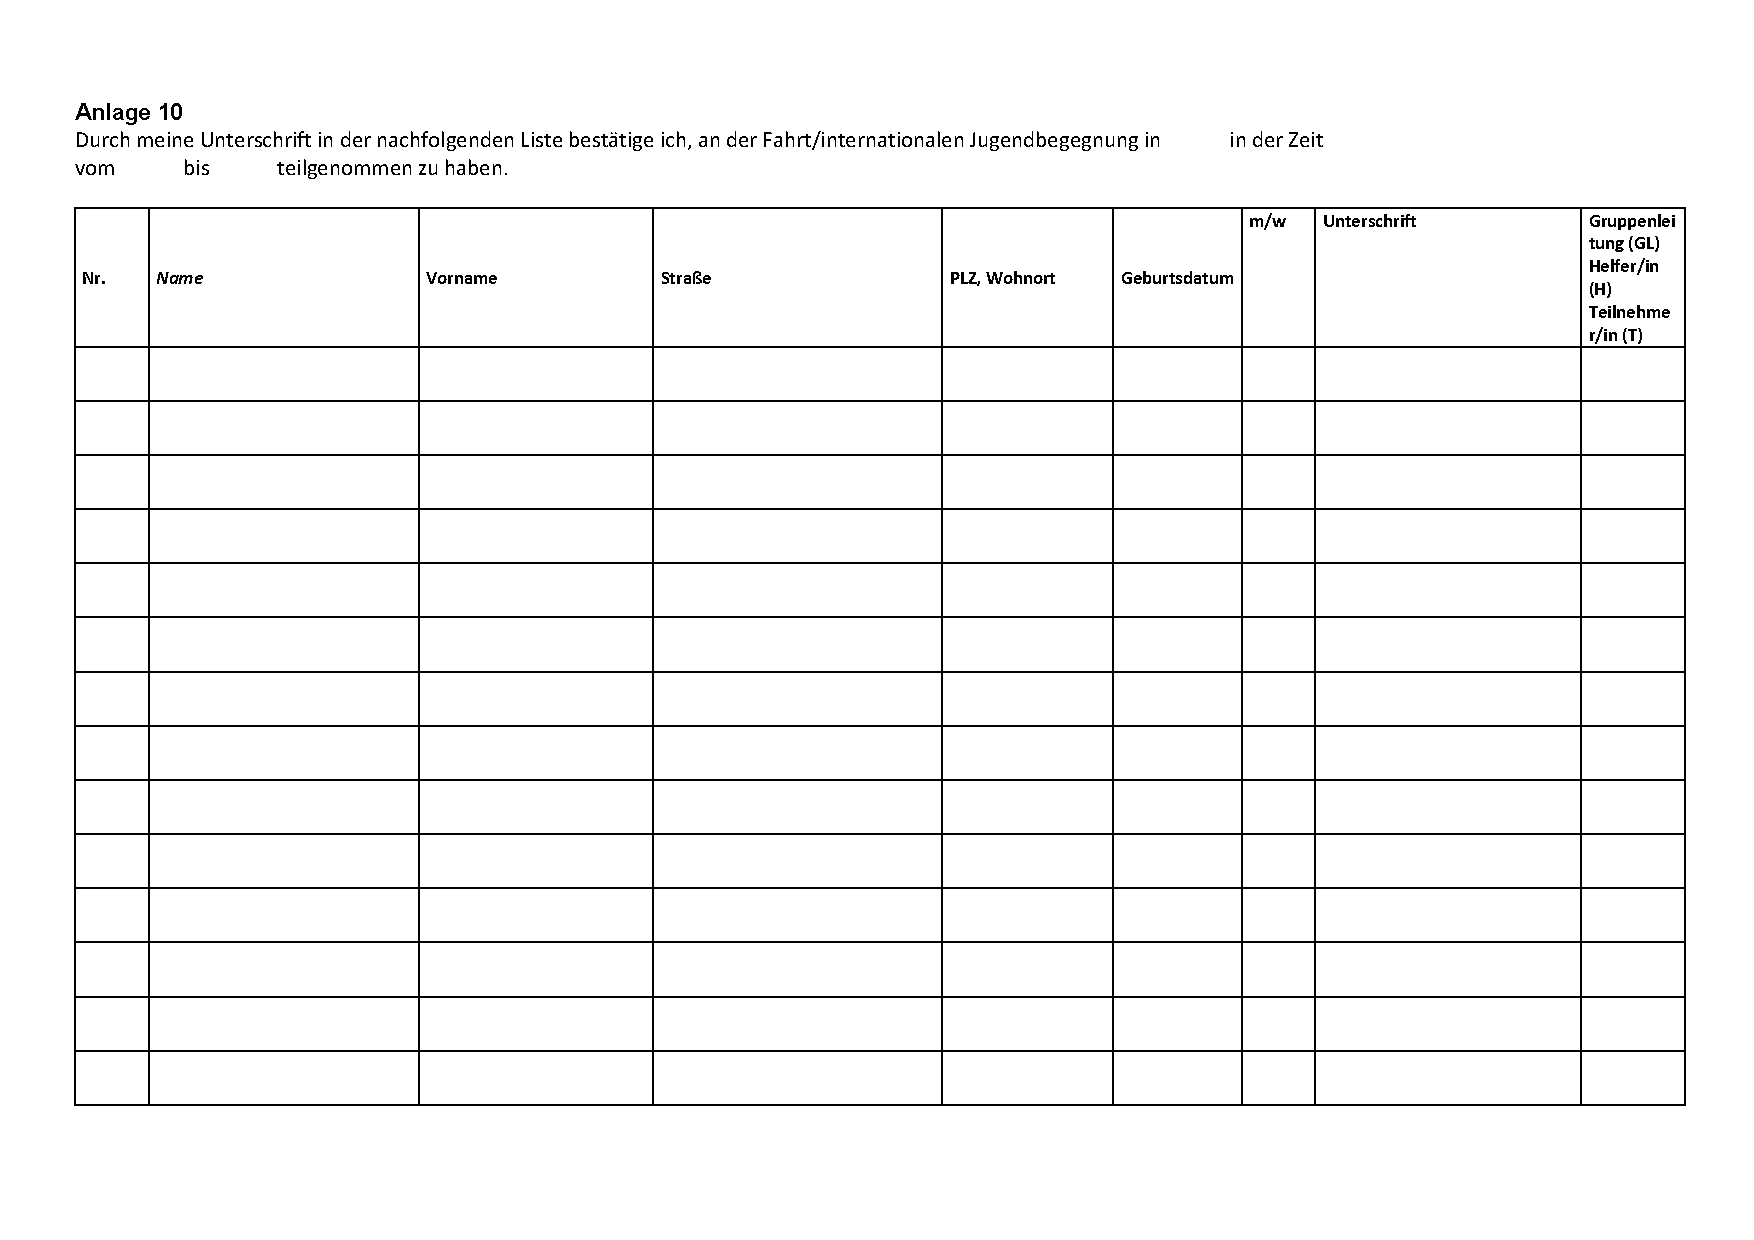
\includegraphics[width = \paperwidth, height = \paperheight] {gallier.pdf}}}

\begin{document}
\noindent \sffamily

@foreach($members as $chunk)
\begin{tikzpicture}[remember picture,overlay,yscale=-1]
\node[anchor=base west] at (17mm,29.62mm) {\bfseries{\small{<<<$dateFromHuman>>>}}};
\node[anchor=base west] at (34mm,29.62mm) {\bfseries{\small{<<<$dateUntilHuman>>>}}};
\node[] at (203mm,15.55mm) {\bfseries{\small{<<<$zipLocation>>>}}};

\node[thick, cross out,draw=black,text width=2.4mm, text height=2.4mm, inner sep=0mm] at (17.76mm,47.10mm) {};

@foreach($chunk as $i => $member)
    \node[anchor=center, text width=9.75mm, align=center] at ($(19.35mm, 59.7mm + 9.2mm * <<<$i%14>>>)$) {<<<$i+1>>>};
    \node[anchor=center, text width=41.75mm, align=center] at ($(48.35mm, 59.7mm + 9.2mm * <<<$i%14>>>)$) {<<<$member->lastname>>>};
    \node[anchor=center, text width=37.75mm, align=center] at ($(91.35mm, 59.7mm + 9.2mm * <<<$i%14>>>)$) {<<<$member->firstname>>>};
    \node[anchor=center, text width=45.75mm, align=center] at ($(135.35mm, 59.7mm + 9.2mm * <<<$i%14>>>)$) {<<<$member->address>>>};
    \node[anchor=center, text width=26.75mm, align=center] at ($(174.35mm, 59.7mm + 9.2mm * <<<$i%14>>>)$) {<<<$member->city()>>>};
    \node[anchor=center, text width=19.75mm, align=center] at ($(199.35mm, 59.7mm + 9.2mm * <<<$i%14>>>)$) {<<<$member->birthdayHuman()>>>};
    \node[anchor=center, text width=7.75mm, align=center] at ($(216.35mm, 59.7mm + 9.2mm * <<<$i%14>>>)$) {<<<$member->gender?->short>>>};
    \node[anchor=center, text width=7.75mm, align=center] at ($(276.35mm, 59.7mm + 9.2mm * <<<$i%14>>>)$) {<<<$member->isLeader ? 'GL' : 'T'>>>};
@endforeach

\end{tikzpicture}

\pagebreak

@endforeach
\end{document}

